\chapter{Uwzgl�dnianie pomiaru zak��ce� w pracy regulatora DMC}
Dob�r parametru $D_z$ jest dobierany analogicznie jak parametry algorytmu DMC w zadaniu 4. Funkcja pozwalaj�ca na ocen� na jako�� regulacji i przebieg warto�ci zadanej s� takie same jak w zadaniu 4. Parametr $D_z$ = 0 oznacza, �e algorytm DMC nie uwzgl�dnia zak��ce� przy obliczaniu sygna�u steruj�cego.

\begin{center}
\begin{figure}[H]
\makebox[\textwidth]{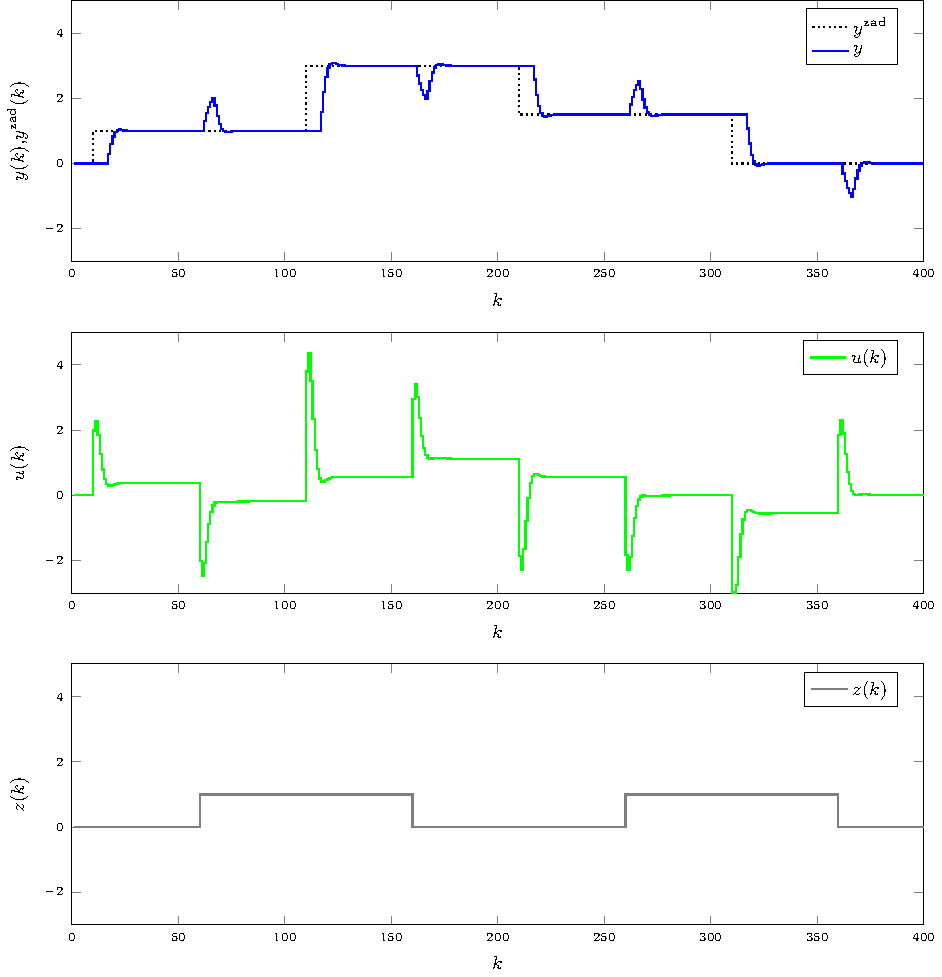
\includegraphics[width=\paperwidth]{data/exercise_4/Desired_output_plot_zad_5_iter_01_D_180_Dz_40_N_20_Nu_10_lambda_0.1_error_87.878.pdf}}
\caption{D=180, Dz=40, N=20, Nu=10, $\lambda=0.1$, error=87.878}
\label{Desired_output_plot_zad_5_iter_01_D_180_Dz_40_N_20_Nu_10_lambda_0.1_error_87.878}
\end{figure}
\end{center}
\begin{center}
\begin{figure}[H]
\makebox[\textwidth]{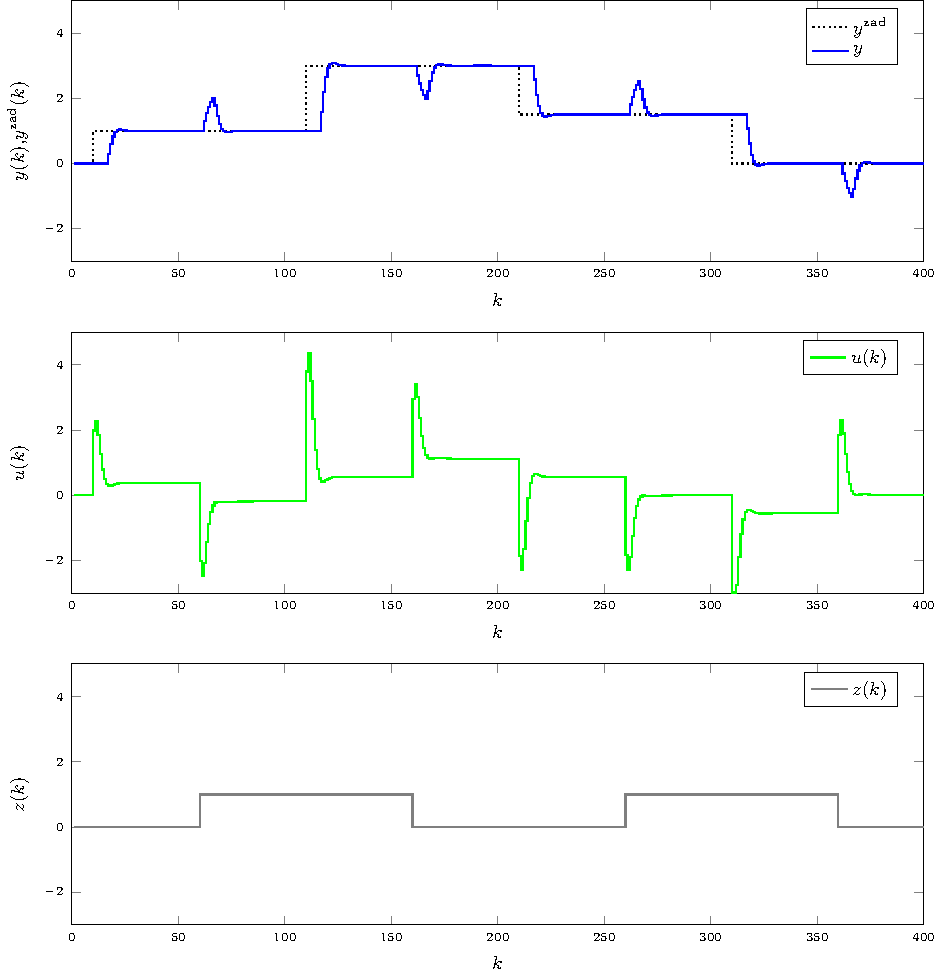
\includegraphics[width=\paperwidth]{data/exercise_4/Desired_output_plot_zad_5_iter_02_D_180_Dz_30_N_20_Nu_10_lambda_0.1_error_87.8781.pdf}}
\caption{D=180, Dz=30, N=20, Nu=10, $\lambda=0.1$, error=87.8781}
\label{Desired_output_plot_zad_5_iter_02_D_180_Dz_30_N_20_Nu_10_lambda_0.1_error_87.8781}
\end{figure}
\end{center}
\begin{center}
\begin{figure}[H]
\makebox[\textwidth]{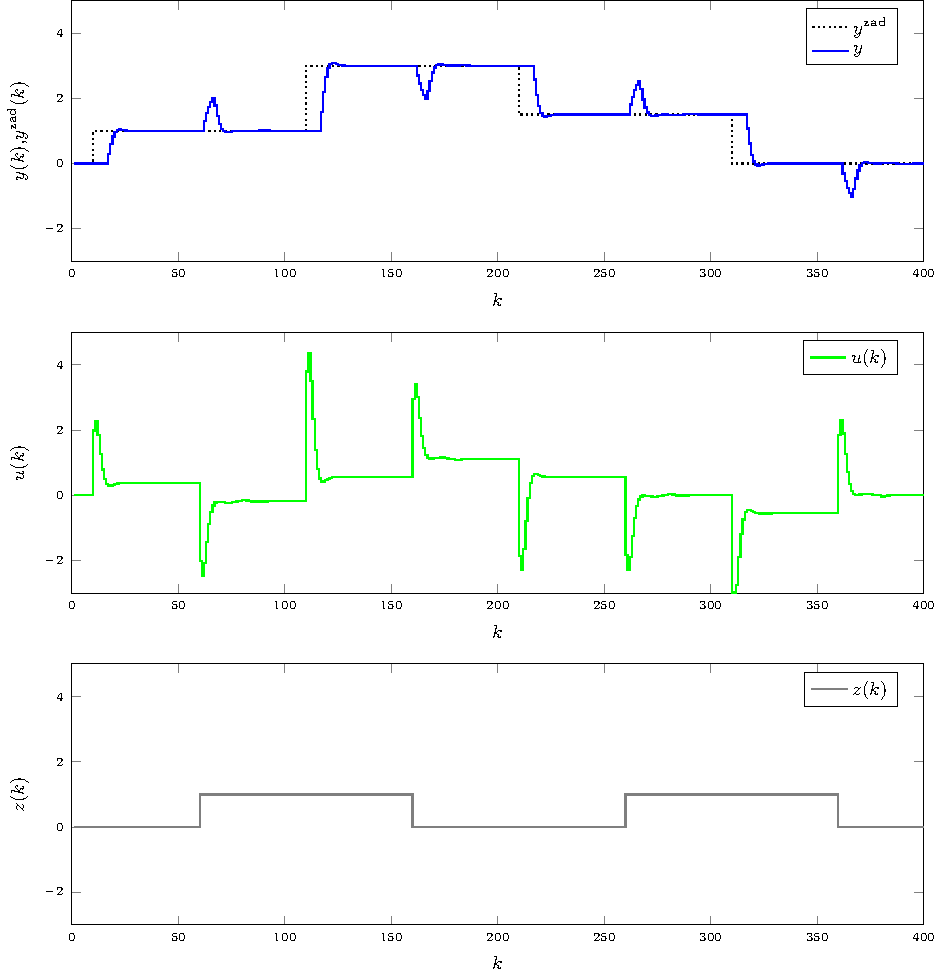
\includegraphics[width=\paperwidth]{data/exercise_4/Desired_output_plot_zad_5_iter_03_D_180_Dz_20_N_20_Nu_10_lambda_0.1_error_87.8816.pdf}}
\caption{D=180, Dz=20, N=20, Nu=10, $\lambda=0.1$, error=87.8816}
\label{Desired_output_plot_zad_5_iter_03_D_180_Dz_20_N_20_Nu_10_lambda_0.1_error_87.8816}
\end{figure}
\end{center}
\begin{center}
\begin{figure}[H]
\makebox[\textwidth]{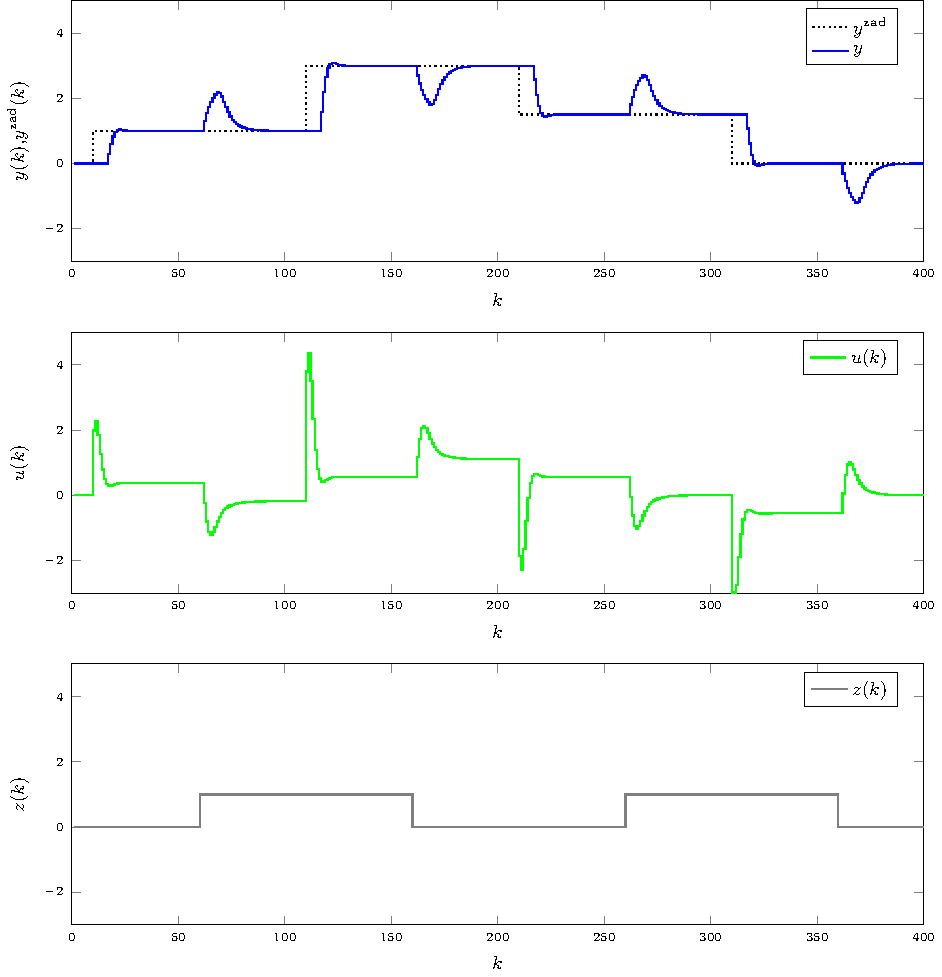
\includegraphics[width=\paperwidth]{data/exercise_4/Desired_output_plot_zad_5_iter_04_D_180_Dz_0_N_20_Nu_10_lambda_0.1_error_113.632.pdf}}
\caption{D=180, Dz=0, N=20, Nu=10, $\lambda=0.1$, error=113.632}
\label{Desired_output_plot_zad_5_iter_04_D_180_Dz_0_N_20_Nu_10_lambda_0.1_error_113.632}
\end{figure}
\end{center}

Jak widzimy zmiana $D_z$ nie ma du�ego wp�ywu na jako�� regulacji, dlatego zmniejszamy t� warto�� aby zmniejszy� liczb� potrzebnych oblicze� w ka�dej iteracji. Wybieramy warto�� 20. Je�eli por�wnamy jako�� regulacji z w��czonym i wy��czonym uwzgl�dnianiem zak��ce� przy wyliczaniu sygna�u steruj�cego to r�nica jest znacz�ca ( oko�o 26 ).